% Name: Intervals on a number line
% Description: The set [-2, 1) ∪ (3, ∞) on a number line: a closed dot where an end is included, an open one where it is not.
% Tags: number line, intervals, inequalities, sets

\usetikzlibrary{arrows.meta}

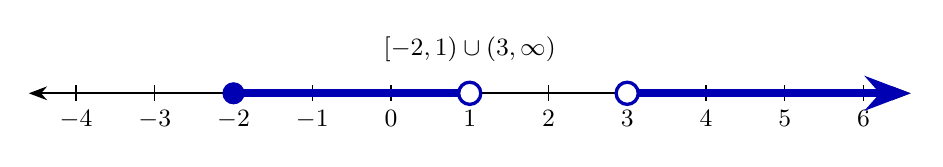
\begin{tikzpicture}[>={Stealth}, every node/.style={font=\small}]
  \draw[<->, thick] (-4.6,0) -- (6.6,0);
  \foreach \x in {-4,...,6} \draw (\x,0.1) -- (\x,-0.1) node[below] {$\x$};
  \draw[line width=3pt, blue!70!black] (-2,0) -- (1,0);
  \draw[->, line width=3pt, blue!70!black] (3,0) -- (6.6,0);
  \fill[blue!70!black] (-2,0) circle (4pt);
  \draw[blue!70!black, very thick, fill=white] (1,0) circle (4pt);
  \draw[blue!70!black, very thick, fill=white] (3,0) circle (4pt);
  \node[above=5pt] at (1,0.1) {$[-2, 1) \cup (3, \infty)$};
\end{tikzpicture}
